\section{La structure d'accueil : le Lab-STICC}
        \paragraph*{}
		Le Lab-STICC\cite{labSticc}, CNRS UMR 6285, est le Laboratoire des Sciences et Techniques de l'Information, de la Communication et de la Connaissance. Il est présent sur les villes de Brest, Quimper, Lorient et Vannes. Il est rattaché à l'Institut des Sciences de l'Information et de leurs Interactions (INS2I) et à l'Institut des Sciences de l'Ingénierie et des Systèmes (INSIS) du CNRS.
		Les pôles du laboratoire sont définis comme des entités permettant d’établir une cohérence scientifique sur les grands domaines couverts par le Lab-STICC tels que par exemple : l'IA et l'Océan, les Systèmes Photoniques et les Hyperfréquences, CyberSécurité et les Réseaux ou encore les Intéractions entre les Systèmes Humains - Machines . Il existe 9 pôles différents au sein du laboratoire.
		
		J'étais assigné au sein du pôle CyR  (Cyber et Réseaux) et de l'équipe IRIS (Sécurité et Résilience des Systèmes d'Information).
		
		\begin{figure}[H]
		    \centering
		    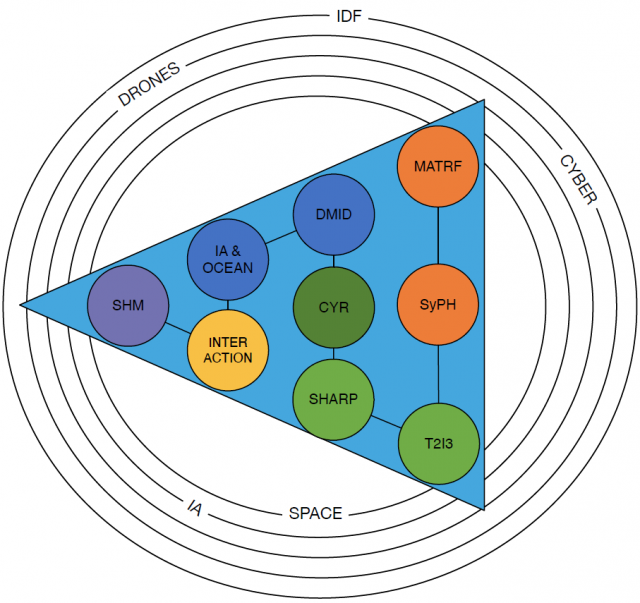
\includegraphics[width=10cm]{image/structLabSTICC.png}
		    \caption{Structure du Lab-STICC avec les différents pôles existants}
		    \label{fig:structLabSTICC}
		\end{figure}